\documentclass[titlepage,a4paper]{article}
\usepackage[a4paper,includeheadfoot,margin=2.54cm]{geometry}
\usepackage{graphicx}
\usepackage{listings}
\usepackage{glossaries}
\makeglossaries
\usepackage{cleveref}
\graphicspath{{img/}}

\newcommand\imgwidth{0.5\textwidth}
\newcommand\centrefigurestart{\begin{figure}[h]\begin{center}}
\newcommand\centrefigureend{\end{center}\end{figure}}

\newacronym{sdr}{SDR}{Software Defined Radio}
\newacronym{RF}{RF}{Radio Frequencies}
\newacronym{mitm}{MITM}{man in the middle}

\begin{document}
\title{Work Experience - RF Guide}
\author{Patrick Mintram}
\maketitle

\tableofcontents
\listoffigures
\printglossaries
\newpage

\section{Introduction}
This guide has been produced to help you work through the \gls{RF} workshop as part of your work experience. In this workshop you will learn \begin{enumerate}\item What things use \gls{RF}. \item How we can make something that uses \gls{RF}. \item How using \gls{RF} can expose your projects to vulnerabilities. \item What tools we can use to help when using \gls{RF}.\end{enumerate}

\subsection{What you will be doing}
In following this workshop you will be using tools available at home, to look at some of the information being sent through the air as \gls{RF}. You will be able to see the different frequencies used by different kinds of devices, such as doorbells, WiFi, remote control cars and bluetooth connected items. You will then send some secret messages between some microcontrollers and use these tools to spy on the message as part of a \gls{mitm} attack.

\subsection{Using this guide}
There may part of this guide which aren't explained very in depth, that is because the subject of \gls{RF} and signals is really complicated, so the detail has been left out. If you want to find out more there are some good overviews available online\footnote{http://www.ti.com/lit/ml/slap127/slap127.pdf, for example}. This guide is meant at more of a practical workshop than an academic exercise, so if something is glossed over a useful link will be provided in the footnotes, as you have already seen. It isn't expected that you full understand the subjects covered, but it is expected that you'll take some time in the future to have a play with the tools and techniques and learn a bit more about the things you've touched on.

\cfbox{red}{ Text in red boxes are things you need to type in. }

\cfbox{blue}{ Text in blue boxes are instructions, but you might not have to type them in. }

\subsection{Feedback}
The author of this guide is keen to know what you think; the good, the bad and the ugly. Please feel free to send any comments their way, or if you're that way inclined, use the github system and raise an issue or create a pull request. 

\newpage

\section{Equipment}
In order to complete this guide you will need the following equipment.

\begin{enumerate}
\item Laptop with the following: 
\begin{enumerate}
\item The \gls{sdr} Drivers. These are usually available from the manufacturers website.
\item The Arduino IDE\footnote{https://www.arduino.cc/en/Main/Software}.
\item The RadioHead-Extras library should be installed and made available to the Arduino IDE. The library is in the \verb|src| folder of this repo.
\item gnuradio\footnote{https://www.gnuradio.org}.
\item A clone of this repo and performed recursively\footnote{git clone --recursive https://github.com/geekskick/wex-guide}.
\end{enumerate}
\item An SDR with an appropriate antenna for looking at the 430-440MHz frequency range. Its up to you which you use, there are loads available for a reasonable price\footnote{https://www.rtl-sdr.com}.
\item Two Adafruit Feathers with an RFM69 packet radio module attached\footnote{https://learn.adafruit.com/adafruit-feather-m0-radio-with-rfm69-packet-radio/overview} as shown in \cref{adafruit}. These should ideally have antennas attached as described in the Adafruit documentation\footnote{https://learn.adafruit.com/adafruit-feather-m0-radio-with-rfm69-packet-radio/antenna-options}. 

\centrefigurestart
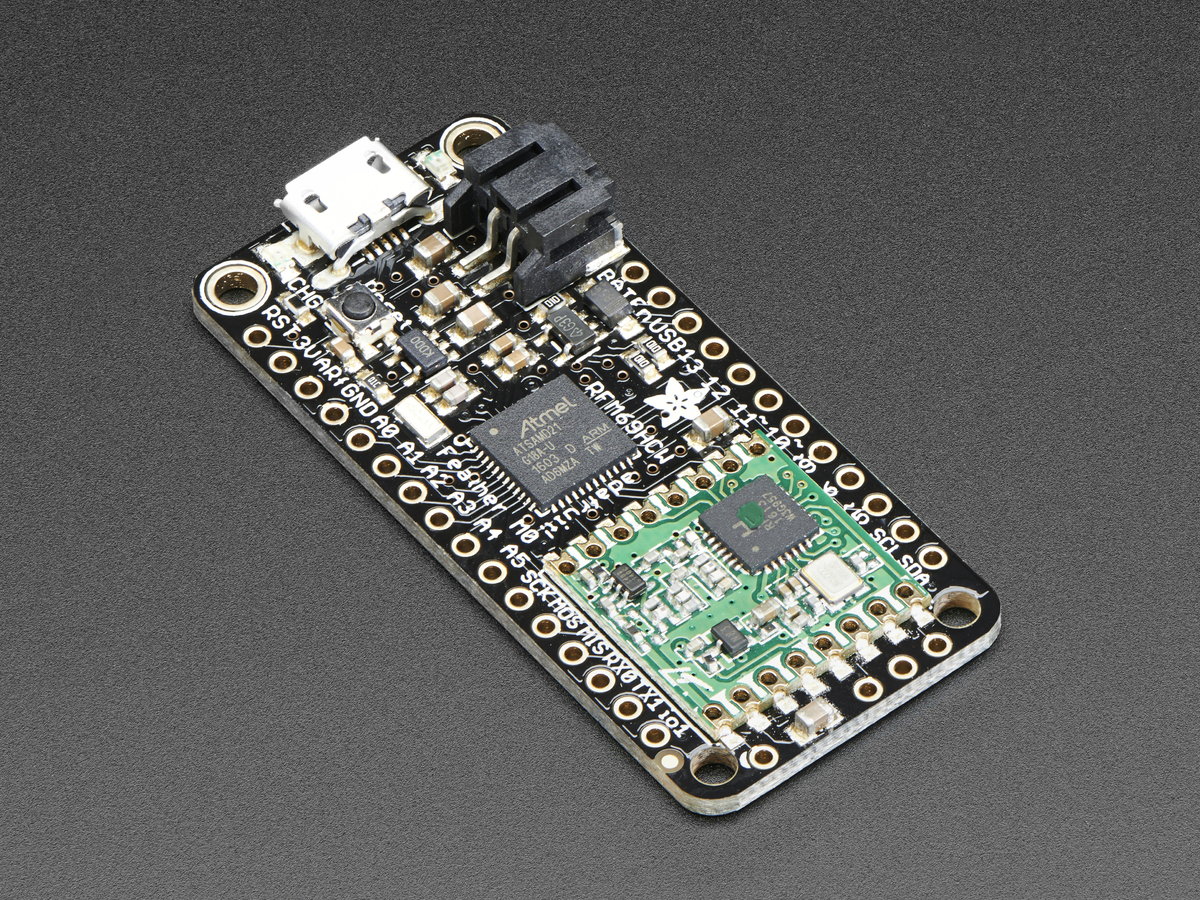
\includegraphics[width=\imgwidth]{feather.jpg}
\caption{An Adafruit Feather M0 with RFM69 Packet Radio}
\label{adafruit}
\centrefigureend

\end{enumerate}
\newpage

\section{Looking at the Spectrum}
Basic gnuradio
\newpage

\section{Sending a secret message}
Feathers
\newpage

\section{Spying on a secret message}
gnuradio
\newpage

\section{Real World Example}
RTL-SDR car stuff
\newpage

\end{document}
